\documentclass[12pt]{article}
\usepackage{polski}
\usepackage[utf8]{inputenc}
\usepackage{graphicx}
\usepackage{amsmath}
\usepackage{graphicx}
\usepackage{setspace}
\usepackage{pdfpages}


\title{ Sprawdzanie prawa Malusa \\
    \large Informatyka – profil praktyczny, semestr II \\
    Wydział Matematyki Stosowanej \\
    Politechnika Śląska \\}

\author{ Sekcja 5 \\
    Piotr Skowroński, Bartłomiej Pacia}
\date{Maj 2022}

\begin{document}

\maketitle

\section{Wstęp teoretyczny}

Falą elektromagnetyczną nazywamy zaburzenie pola elektromagnetycznego
rozchodzące się w przestrzeni. Zmienne pole elektryczne wytwarza pole
magnetyczne. Z kolei zmienne pole magnetyczne wytwarza pole elektryczne.
Oznacza to, że fala elektromagnetyczna to inaczej sprzężone ze sobą
pola elektryczne i magnetyczne. Fala elektromagnetyczna jest
przykładem fali poprzecznej.

Fala poprzeczna to fala, w której oscylacje są
prostopadłe do kierunku rozchodzenia się tej fali. Polaryzacja
jest zjawiskiem możliwym tylko dla fali poprzecznej. W przypadku
fali niespolaryzowanej fala oscyluje we wszystkich możliwych
kierunkach prostopadłych do kierunku rozchodzenia się fali. Polaryzacja
jest procesem, w wyniku którego osiągamy tylko jeden kierunek oscylacji.
Możliwe jest to dla światła na przykład przy pomocy tak zwanego
polaryzatora, czyli materiału pochłaniającego światło w kierunku
ułożenia cząsteczek tego materiału.

Prawo Malusa mówi, że natężenie światła spolaryzowanego jest równe
natężeniu światła padającego na polaryzator pomnożonemu przez cosinus
kąta padania tego światła do kwadratu. Prawo to działa, tylko kiedy
światło padające jest spolaryzowane.

\begin{center}
    $I = I_0 \cdot \cos^2(\phi)$ \\
\end{center}
Gdzie: \\
\indent $I$ - natężenie światła spolaryzowanego,\\
\indent $I_0$ - natężenie światła padającego, \\
\indent $\phi$ - kąt między płaszczyzną polaryzacji
światła a płaszczyzną polaryzacji polaryzatora. \\
Celem ćwiczenia jest sprawdzenie, czy prawo Malusa zachodzi.

\section{Pomiary}

Podczas wykonywania doświadczenia w pracowni pomiary zapisywaliśmy ręcznie na
kartce. Następnie przepisaliśmy wyniki naszych pomiarów do pliku CSV, by
umożliwić ich wykorzystanie w programie.

Użyliśmy języka Python w środowisku Jupyter Notebook. Wykorzystaliśmy biblioteki
\textit{numpy}, \textit{pandas} i \textit{matplotlib}.
\section{Wykresy i tabelka z danymi}

\subsection*{Wykres $I(\phi)$, $I_T(\phi)$, Obrócony wykres
    $I_T(\phi + \alpha)$ i tabelka z obliczeniami}
Przyjmujemy niepewności: \\
\indent $u(\phi) = 0.5 ^{\circ}$, \\
\indent $u(I) = \frac{0.8\% \cdot I + 0.2}{\sqrt{3}}$ dla użytego przez nas urządzenia, \\
\indent $u(I_T) = \sqrt{(2I_{max}\cos(\phi)\sin(\phi) \cdot u(\phi))^2 + (\cos(phi) \cdot u(I))^2}$
Z prawa przenoszenia niepewności, \\
\indent Kąt obrotu $\alpha = 110^{\circ}$. \\
Wykresy na następnych stronach.
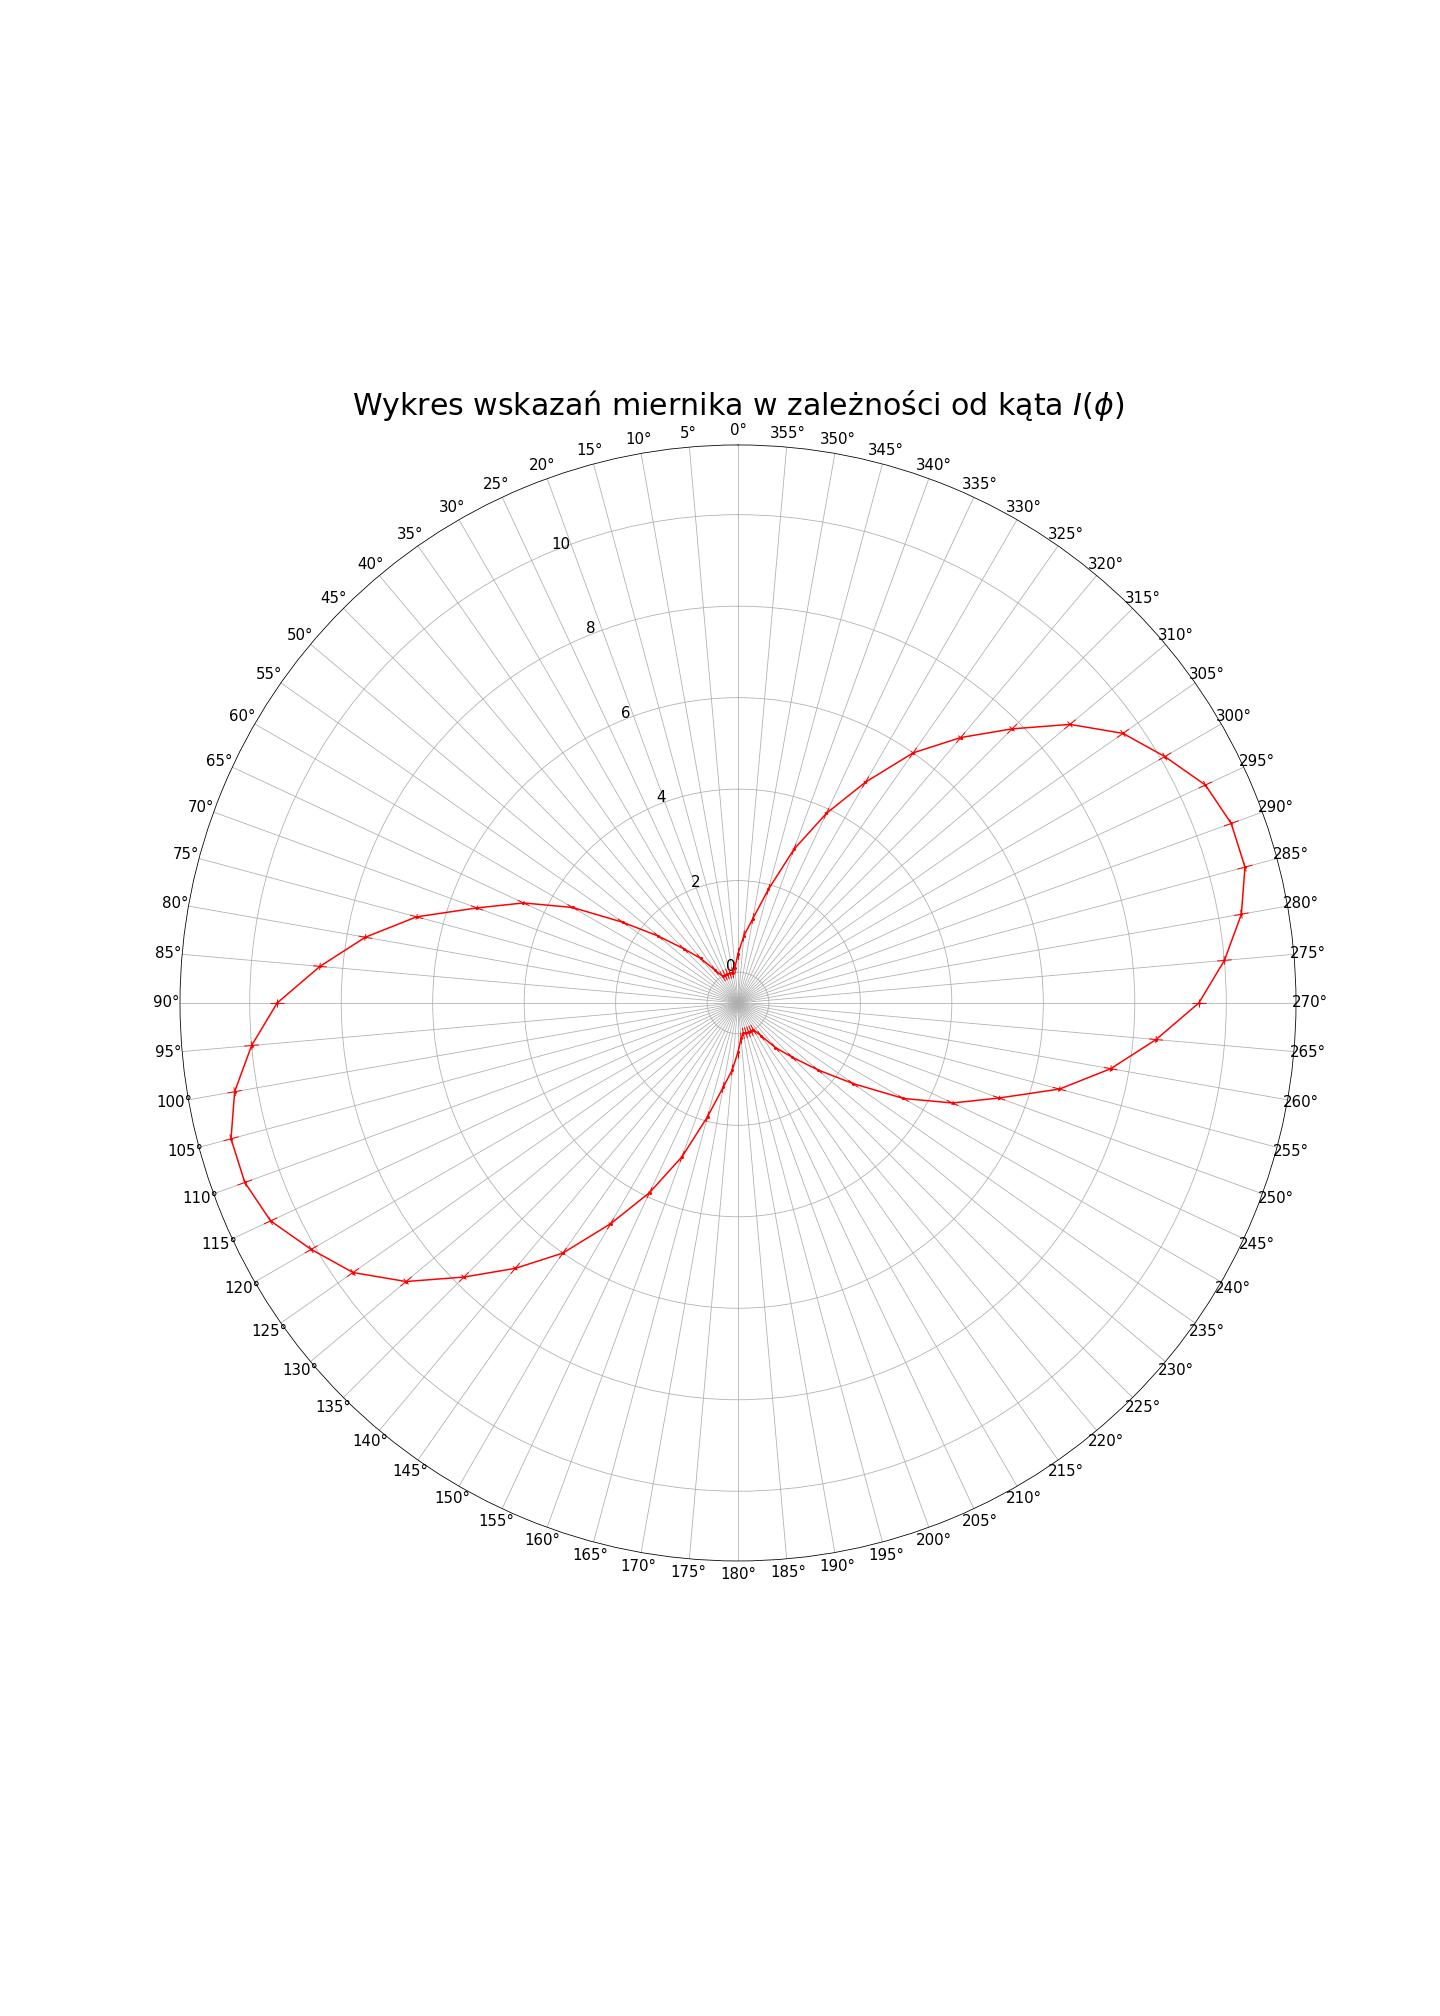
\includepdf{"./img/wykres1.jpg"}
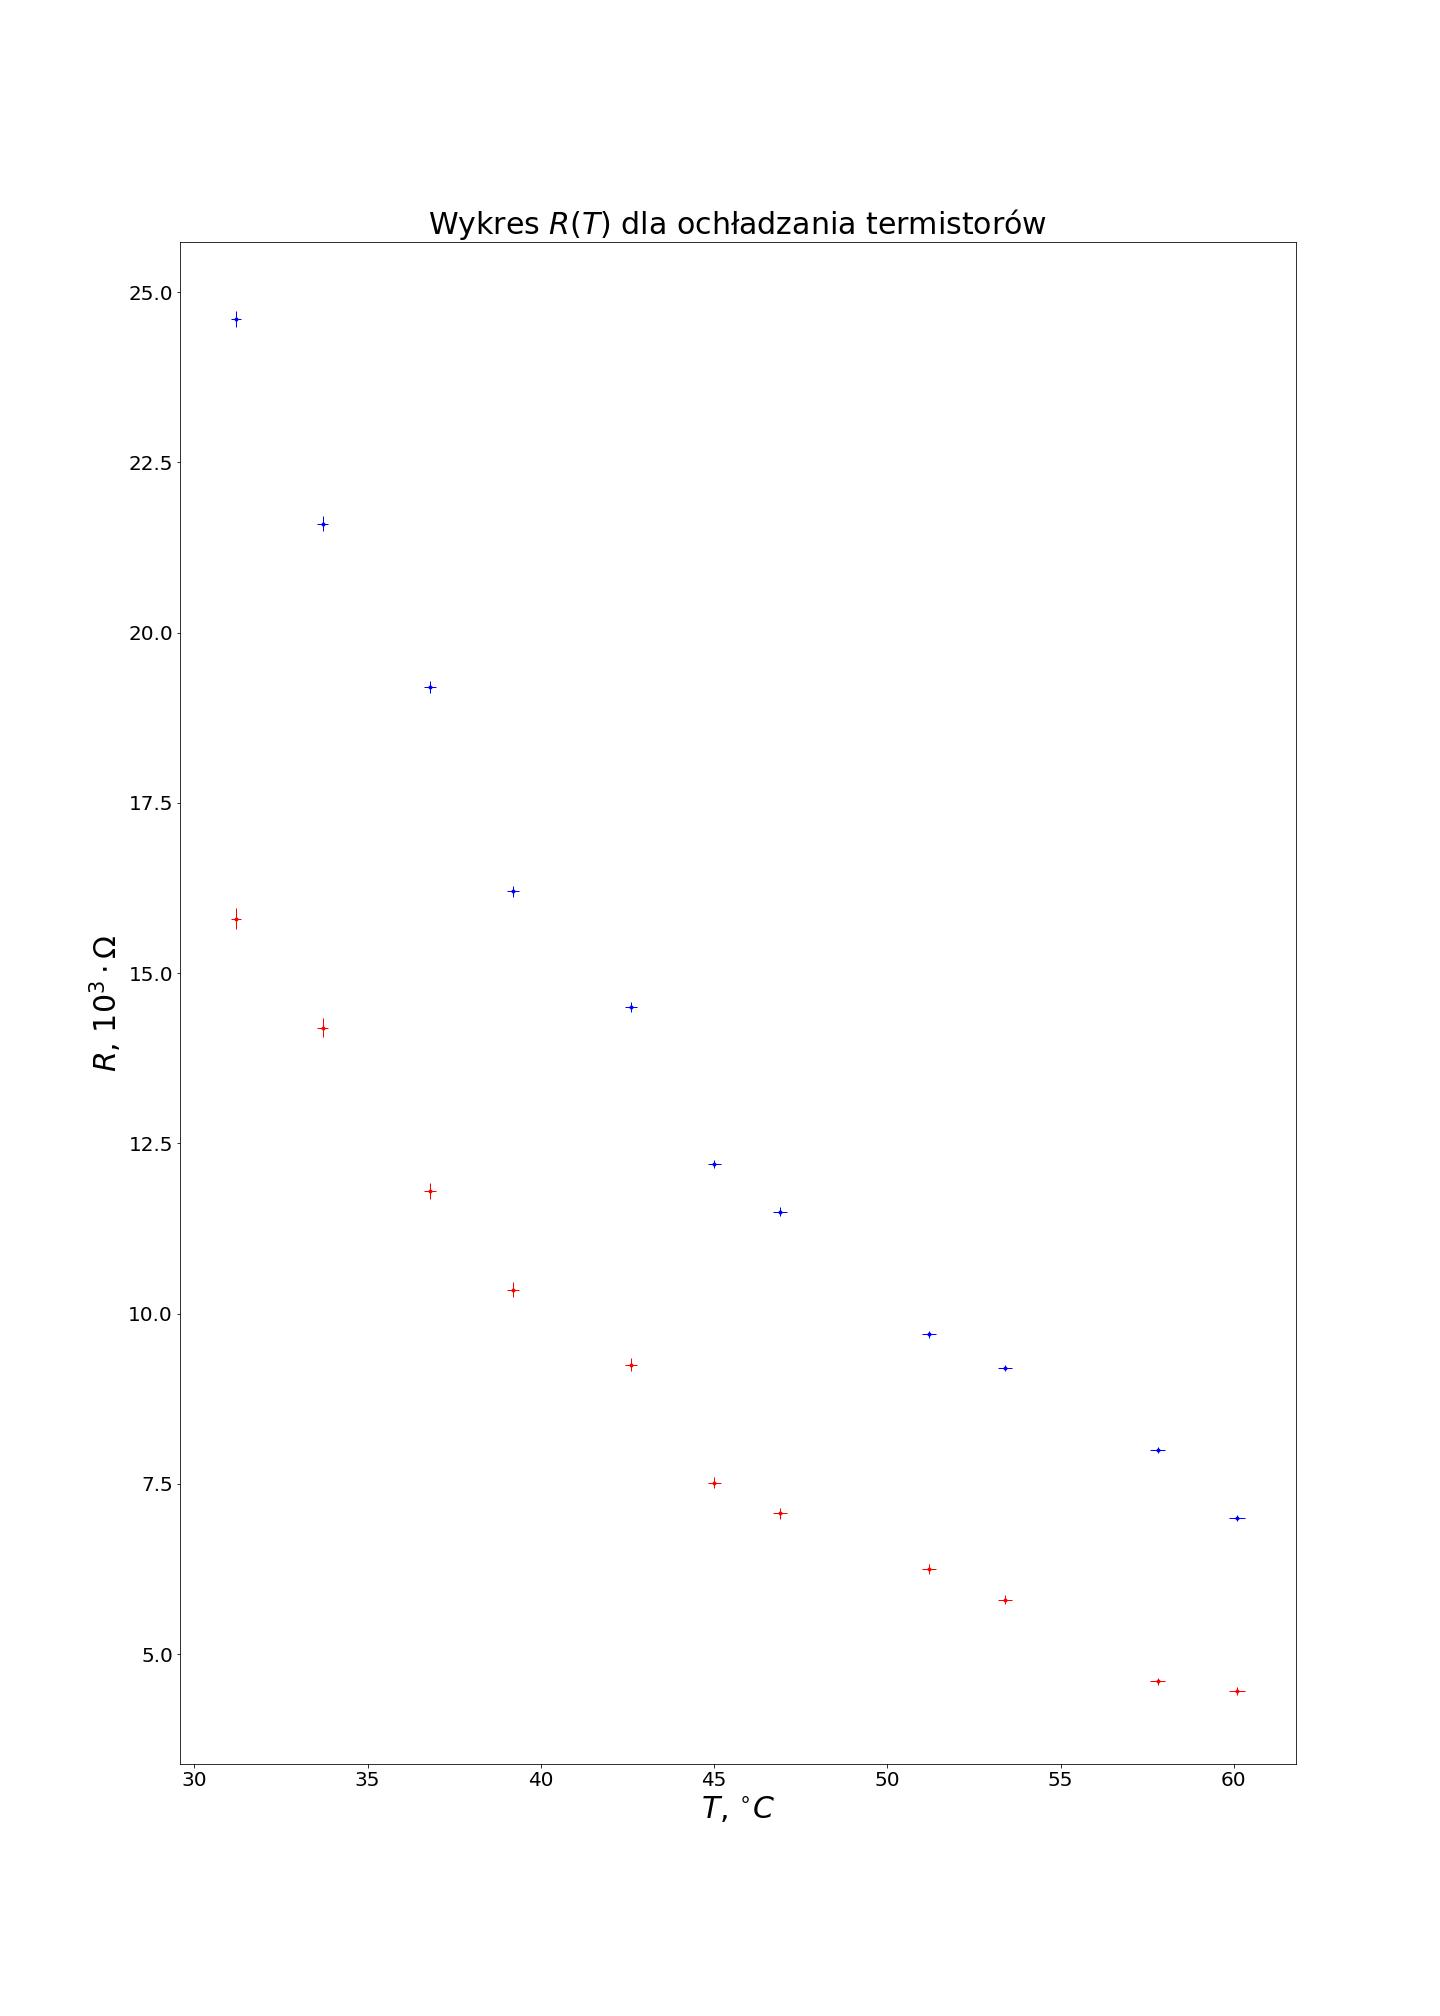
\includepdf{"./img/wykres2.jpg"}
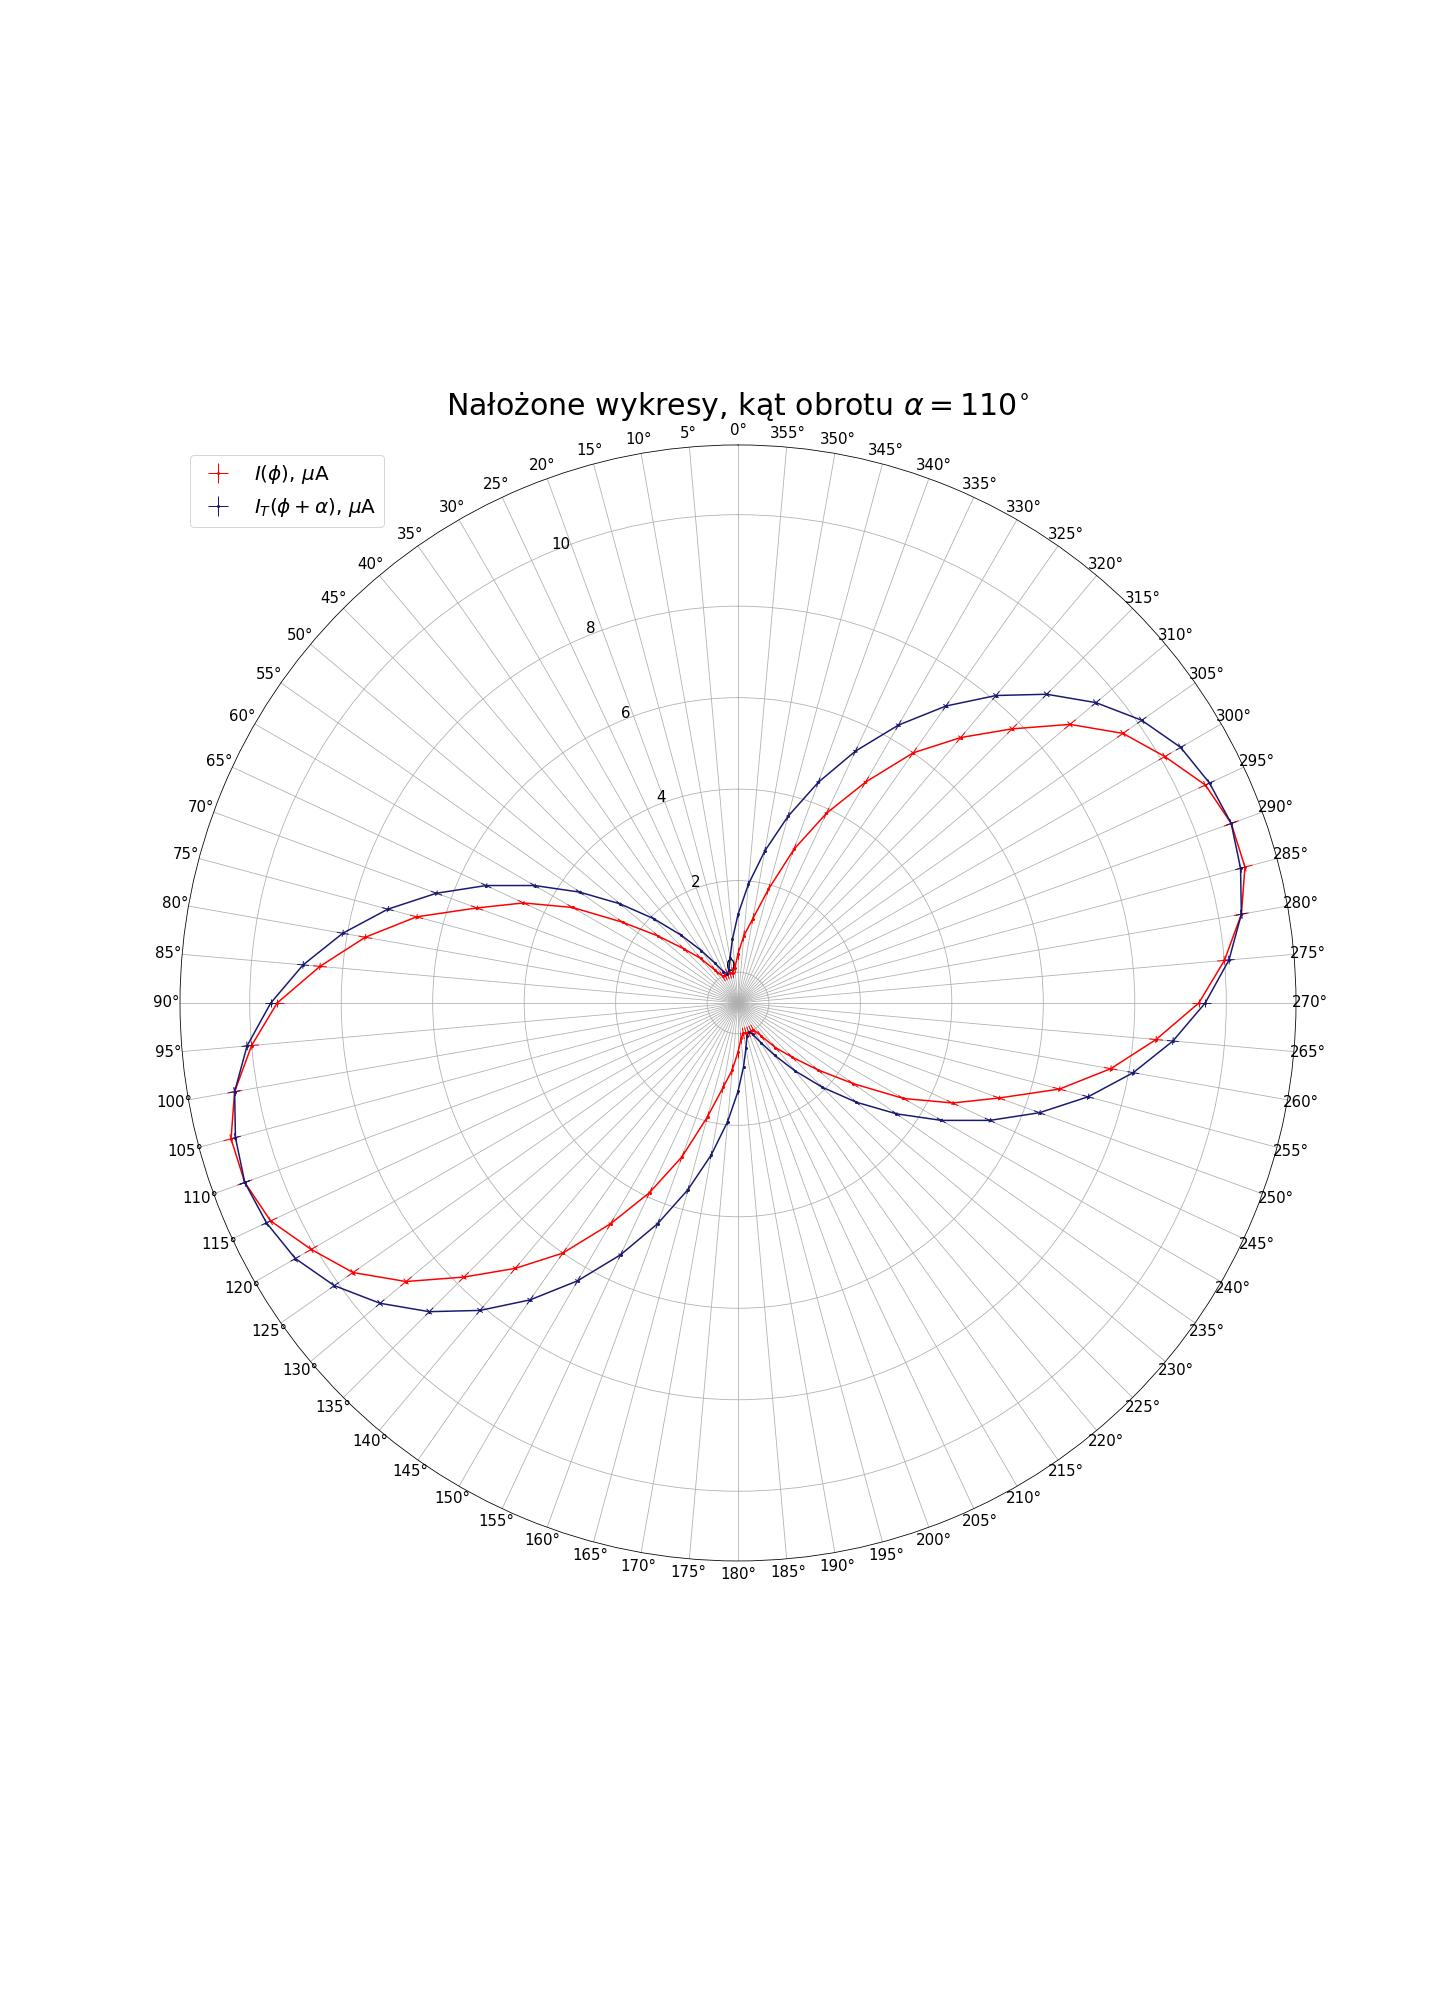
\includepdf{"./img/wykres3.jpg"}

\subsection*{Tabelka z danymi}
\begin{center}
    \begin{tabular}{*{5}{| c |}}
        \hline
        $\phi$, $^{\circ}$ & $I_0$, $\mu$A & $I_T$, $\mu$A & $u(I_0)$, $\mu$A & $u(I_T)$, $\mu$A \\ \hline
        0                  & 0.40          & 10.80         & 0.12             & 0.12             \\ \hline
        5                  & 0.10          & 10.70         & 0.12             & 0.12             \\ \hline
        10                 & 0.00          & 10.50         & 0.12             & 0.12             \\ \hline
        15                 & 0.00          & 10.10         & 0.12             & 0.12             \\ \hline
        20                 & 0.00          & 9.54          & 0.12             & 0.12             \\ \hline
        25                 & 0.00          & 8.87          & 0.12             & 0.12             \\ \hline
        30                 & 0.00          & 8.10          & 0.12             & 0.12             \\ \hline
        35                 & 0.20          & 7.25          & 0.12             & 0.12             \\ \hline
        40                 & 0.60          & 6.34          & 0.12             & 0.12             \\ \hline
        45                 & 1.00          & 5.40          & 0.12             & 0.11             \\ \hline
        50                 & 1.60          & 4.46          & 0.12             & 0.11             \\ \hline
        55                 & 2.40          & 3.550         & 0.13             & 0.098            \\ \hline
        60                 & 3.50          & 2.700         & 0.13             & 0.088            \\ \hline
        65                 & 4.50          & 1.930         & 0.14             & 0.076            \\ \hline
        70                 & 5.40          & 1.260         & 0.14             & 0.063            \\ \hline
        75                 & 6.60          & 0.723         & 0.15             & 0.048            \\ \hline
        80                 & 7.60          & 0.326         & 0.15             & 0.033            \\ \hline
        85                 & 8.50          & 0.082         & 0.15             & 0.016            \\ \hline
        90                 & 9.40          & 0.00          & 0.16             & 0.00             \\ \hline
        95                 & 10.00         & 0.082         & 0.16             & 0.016            \\ \hline
        100                & 10.50         & 0.326         & 0.16             & 0.033            \\ \hline
        105                & 10.80         & 0.723         & 0.17             & 0.048            \\ \hline
        110                & 10.80         & 1.260         & 0.17             & 0.064            \\ \hline
        115                & 10.60         & 1.930         & 0.16             & 0.078            \\ \hline
        120                & 10.10         & 2.700         & 0.16             & 0.091            \\ \hline
        125                & 9.60          & 3.55          & 0.16             & 0.10             \\ \hline
        130                & 8.80          & 4.46          & 0.16             & 0.11             \\ \hline
        135                & 7.80          & 5.40          & 0.15             & 0.12             \\ \hline
        140                & 6.90          & 6.34          & 0.15             & 0.13             \\ \hline
        145                & 6.00          & 7.25          & 0.14             & 0.13             \\ \hline
        150                & 4.90          & 8.10          & 0.14             & 0.13             \\ \hline
        155                & 3.90          & 8.87          & 0.13             & 0.13             \\ \hline
        160                & 2.90          & 9.54          & 0.13             & 0.13             \\ \hline
        165                & 1.90          & 10.10         & 0.12             & 0.12             \\ \hline
        170                & 1.20          & 10.50         & 0.12             & 0.12             \\ \hline
        175                & 0.80          & 10.70         & 0.12             & 0.12             \\ \hline
        180                & 0.40          & 10.80         & 0.12             & 0.12             \\ \hline
        \hline
    \end{tabular}
\end{center}
\section{Wnioski}
Otrzymane przez nas wykresy pokazują, że prawo Malusa
jest spełnione. Obrócony wykres teoretyczny niemal pokrywa się z
wykresem naszych danych pomiarowych. Błędy pomiarowe wynikają z
niedokładności urządzenia mierzącego natężenie prądu, jak i
niedokładnego odczytu kąta między płaszczyzną polaryzacji światła
a płaszczyzną polaryzacji polaryzatora.
\end{document}
